\tikzset{
	main/.style={black, line width=0.4mm, opacity=1},
	second/.style={gray, opacity=5},
	arrow/.style={-latex, shorten >=1ex, shorten <=1ex, bend angle=45}
}
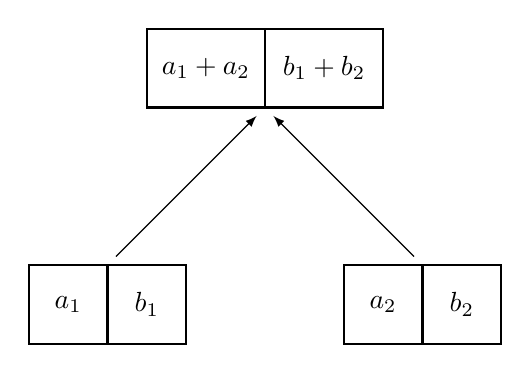
\begin{tikzpicture}

\node (rect) at (1.75,0) [draw,thick,minimum width=1.5cm,minimum height=1cm] {$a_1 + a_2$};
\node (rect) at (3.25,0) [draw,thick,minimum width=1.5cm,minimum height=1cm] {$b_1 + b_2$};


\node (rect) at (0,-3) [draw,thick,minimum width=1cm,minimum height=1cm] {$a_1$};
\node (rect) at (1,-3) [draw,thick,minimum width=1cm,minimum height=1cm] {$b_1$};


\node (rect) at (4,-3) [draw,thick,minimum width=1cm,minimum height=1cm] {$a_2$};
\node (rect) at (5,-3) [draw,thick,minimum width=1cm,minimum height=1cm] {$b_2$};


\draw [arrow]  (0.5,-2.5) to (2.5,-0.5) ;
\draw [arrow]  (4.5,-2.5) to (2.5,-0.5) ;

\end{tikzpicture}